% Appendix Template

\chapter{Appendix B: Structure Retrieval Results} % Main appendix title

\label{AppendixB} % Change X to a consecutive letter; for referencing this appendix elsewhere, use \ref{AppendixB}


\lhead{Appendix B. \emphStructure Retrieval Results} % Change X to a consecutive letter; this is for the header on each page - perhaps a shortened title

\section{Structure Retrieval Results}
\label{sec:mfccappen}

\begin{figure}[b]
    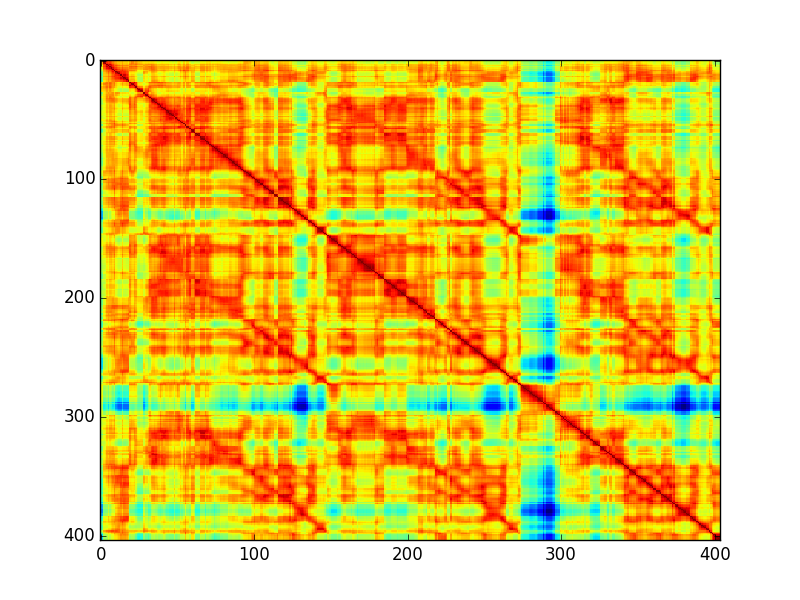
\includegraphics[width=0.75\textwidth]{Figures/mfcc_ssm_euclidean}
    \centering

  \caption{Similarity matrix calculated from Mel-frequency Cepstral Coefficients using Euclidean distance.}
  \label{fig:anneval}
\end{figure}


\begin{figure}[t]
    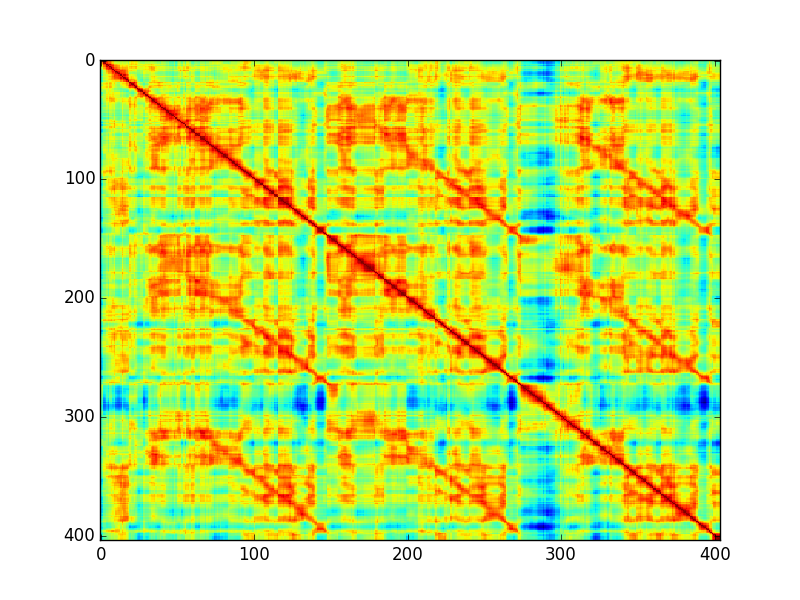
\includegraphics[width=0.75\textwidth]{Figures/mfcc_ssm_manhattan}
    \centering

  \caption{Similarity matrix calculated from Mel-frequency Cepstral Coefficients using Manhattan distance.}
  \label{fig:anneval}
\end{figure}


\begin{figure}[b]
    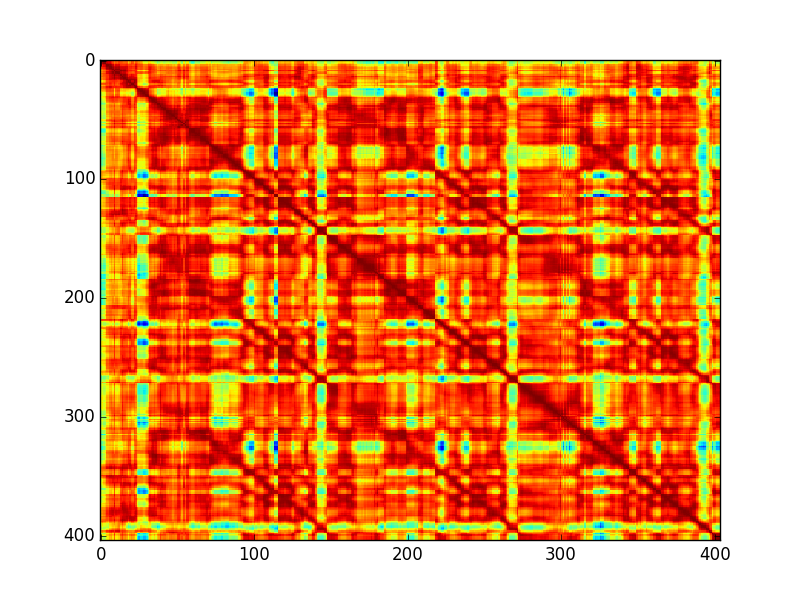
\includegraphics[width=0.75\textwidth]{Figures/mfcc_ssm_cosine}
    \centering

  \caption{Similarity matrix calculated from Mel-frequency Cepstral Coefficients using cosine distance.}
  \label{fig:anneval}
\end{figure}
